\section{E3: Changing the model}
\renewcommand{\Ex}{E3}
Up to this point, all experiments have employed the observation and state space models outlined in the introduction of the Experiments section (see \ref{sec:experiments}). However, using these models in scenarios presented by videos \textit{V1, V2, V3} comes with several disadvantages. The state space model assumes uniform position uncertainty in all directions for targets. Additionally, the videos are not captured from a bird's-eye view but from an angled perspective. This camera angle causes detected targets to appear smaller when they are farther away and larger when they are closer to the camera. Consequently, this effect alters the actual movement model of the targets, which our current model does not account for.


Considering the videos utilized in this study, we can leverage prior knowledge regarding potential targets, such as cars, movement patterns. It is established that cars are inclined to move in the direction of the road rather than backwards or sideways.
\subsection{V2}
\renewcommand{\Vs}{V2}
For this experiment video \textit{V2} with the added crossing road as an obstacle is used. The video is observed at the rate 14 fps.

The state space CVM model is employed with transition matrix

\begin{align}
    F_k &=
    \begin{bmatrix}
        1 & 0 & 2\Delta & 0\\
        0 & 1 & 0 & \Delta \\
        0 & 0 & 1.1 & 0 \\
        0 & 0 & 0 & 1.1
    \end{bmatrix},
\end{align}
where $\Delta = 1$,
and process covariance matrix
\begin{align}
    Q_k &=
    \begin{bmatrix}
        2 & 0.5 & 0 & 0\\
        0 & 1 & 0 & 0 \\
        0 & 0 & 1 & 0 \\
        0 & 0 & 0 & 1
    \end{bmatrix}
    * 0.003.
    \label{eq:exp_E3-V2_Q}
\end{align}

The observation covariance matrix is reformulated as
\begin{align}
    R_k &=
    \begin{bmatrix}
        2 & 0.5 \\
        0 & 1
    \end{bmatrix}
    * 20.
    \label{eq:exp_E3-V2_R}
\end{align}

The spawning point providing nearby targets with initial covariance matrix $P$ is established as
\begin{align}
    P_k &=
    \begin{bmatrix}
        80 & 20 & 0 & 0 \\
        0 & 40 & 0 & 0 \\
        0 & 0 & 40 & 0 \\
        0 & 0 & 0 & 40
    \end{bmatrix}. \label{eq:exp_E3-V2_P}
\end{align}

These model formulations ensure that the noise covariance takes an ellipsoidal shape rather than a circular one. These ellipses are oriented in the direction of the road, indicating that uncertainty increases more in alignment with the road's direction. This implies a lower probability of a car being positioned next to the road in the subsequent time step.
\subsection{V2b -- GM-PHD with dynamic detection probability}
The GM-PHD filter with the dynamic detection probability is analysed only in this experiment. The best performing settings are used - \textit{S3}, i.e., grounded SAM.

\subsubsection{S3 -- Grounded SAM}
\renewcommand{\Set}{S3}
Note in Table \ref{tab:\Ex-\Vs-\Set}, that the standard pruning threshold $T_p$ is the same as the lowered pruning threshold $T_l$. Due to the better model settings and dynamic detection probability, it is not neccesarry to lower the pruning threshold for targets in \textit{detected} and \textit{hidden} state.
\begin{table}[H]
    \centering
    \begin{tabular}{|c|c|c|c|c|c|c|c|c|c|}
        \hline
        $P_{D,k}(x)$ & $P$ & $\sigma_{\upsilon}$ & $\sigma_{\epsilon}$ & $T_H$ & $T_d$ & $T_p$ & $T_l$ & $T_{text}$ & $T_{bbox}$\\ \noalign{\hrule
        height 1.5pt}
        0.3 & see \ref{eq:exp_E3-V2_P} & see \ref{eq:exp_E3-V2_Q} & see \ref{eq:exp_E3-V2_R} & 0.6 & 3 & 0.1 & 0.1 & 0.3 & 0.3\\
        \hline
    \end{tabular}
    \caption{The parameter settings for experiment {\Ex-\Vs-\Set} with dynamic detection probability.}
    \label{tab:\Ex-\Vs-\Set}
\end{table}

The adjust models project in Figures \ref{fig:\Ex-\Vs-\Set_1} and \ref{fig:\Ex-\Vs-\Set_2}. The spawning point has
ellipsoidal shape, as well as the covariances showing the uncertainty given by the covariance matrix $P$. Two cars
are observed in the sequence. Let us call the car driving in the right highway line in the direction of travel $C_R$
and the left car as $C_L$.

\begin{itemize}
    \item \textbf{\ref{fig:\Ex-\Vs-\Set:01}:} Two targets come closer to the obstacle. Both cars are successfully
    detected and initialized.
    \item \textbf{\ref{fig:\Ex-\Vs-\Set:02}:} The target $C_R$ is detected for the last time before the obstacle.
    \item \textbf{\ref{fig:\Ex-\Vs-\Set:03}:} The object detector is still able to detect $C_L$. However, its
    position is already under the obstacle, thus both targets are in \textit{hidden} state.
    \item \textbf{\ref{fig:\Ex-\Vs-\Set:04}:} Both targets are still hidden, the effect of changed models is obvious. The covariances are elongated in the direction of travel and do not interfer outside of the traffic line.
    \item \textbf{\ref{fig:\Ex-\Vs-\Set:05}:} There was not paying
    much attention for fine tuning the model parameters for this experiment. Still the means of predicted positions
    are almost at the right spot. Both cars are detected again, thus the filter get its measurements.
    \item \textbf{\ref{fig:\Ex-\Vs-\Set:06}:} The false additional target is removed, both targets are tracked with
    small ellipsoidal covariances.
\end{itemize}


\begin{figure}[H]
    \centering
    \begin{subfigure}{\textwidth}
        \centering
        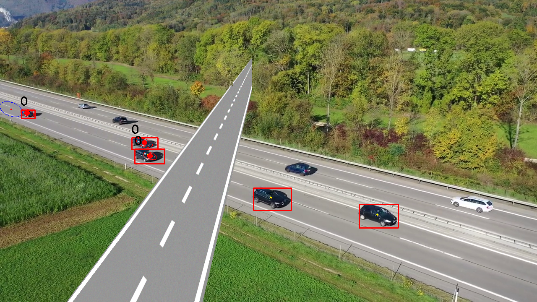
\includegraphics[width=0.85\linewidth]{../../../experiments/\Ex/\Vs/DINO/44}
        \caption{Frame number: 44.}
        \label{fig:\Ex-\Vs-\Set:01}
    \end{subfigure}
    \begin{subfigure}{\textwidth}
        \centering
        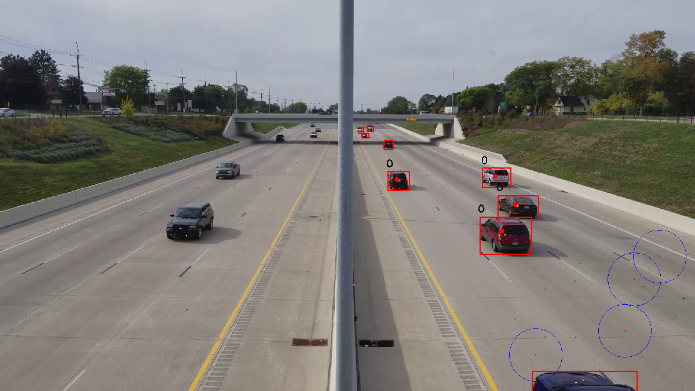
\includegraphics[width=0.85\linewidth]{../../../experiments/\Ex/\Vs/DINO/48}
        \caption{Frame number: 48.}
        \label{fig:\Ex-\Vs-\Set:02}
    \end{subfigure}
    \\
    \begin{subfigure}{\textwidth}
        \centering
        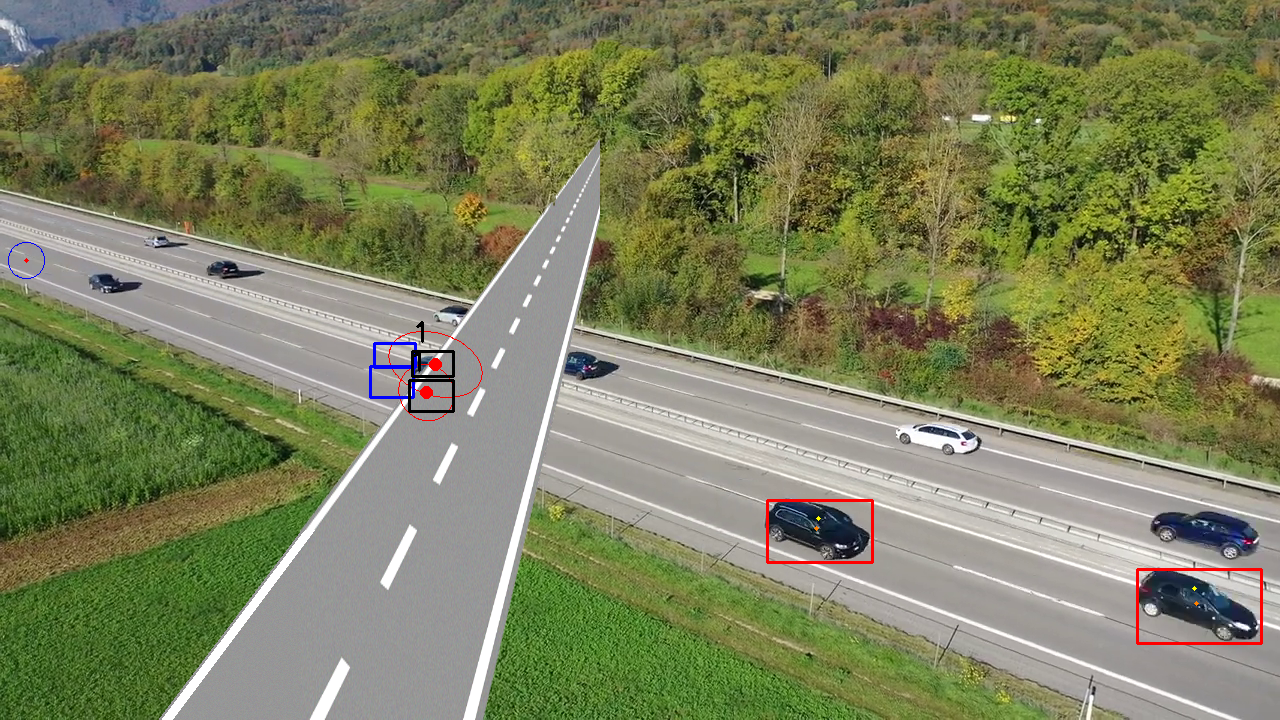
\includegraphics[width=0.85\linewidth]{../../../experiments/\Ex/\Vs/DINO/50}
        \caption{Frame number: 50.}
        \label{fig:\Ex-\Vs-\Set:03}
    \end{subfigure}
    \caption{Image sequence of tracked objects using GM-PHD filter with dynamic detection probability, Grounded SAM and adjusted models -- part 1.}
    \label{fig:\Ex-\Vs-\Set_1}
\end{figure}
\begin{figure}[H]

    \begin{subfigure}{\textwidth}
        \centering
        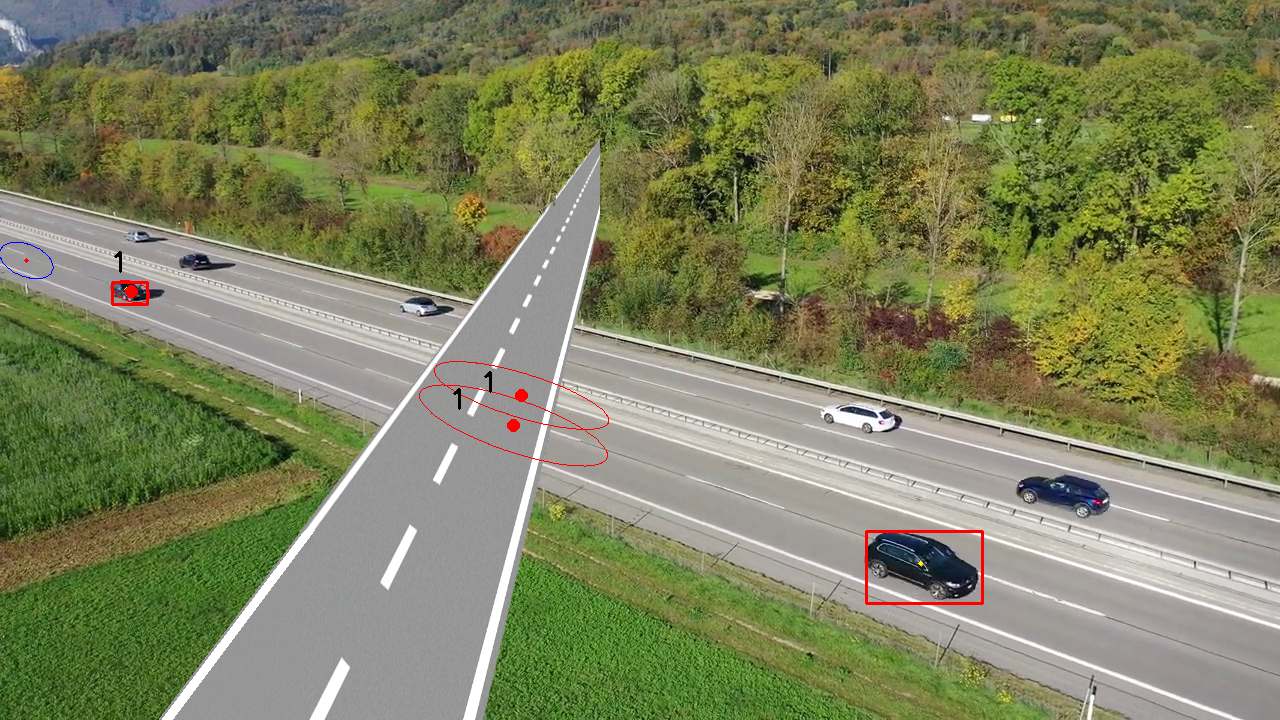
\includegraphics[width=0.85\linewidth]{../../../experiments/\Ex/\Vs/DINO/53}
        \caption{Frame number: 53.}
        \label{fig:\Ex-\Vs-\Set:04}
    \end{subfigure}
    \\
    \begin{subfigure}{\textwidth}
        \centering
        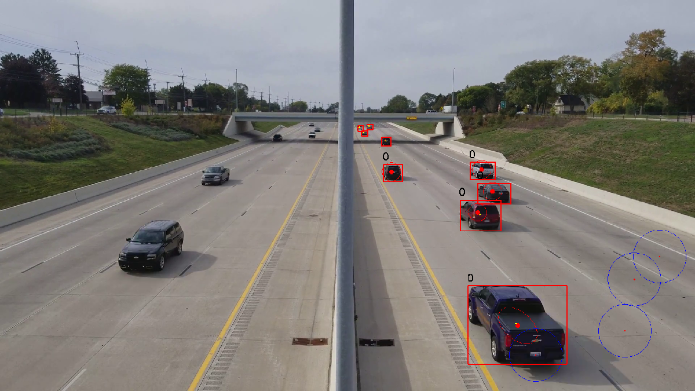
\includegraphics[width=0.85\linewidth]{../../../experiments/\Ex/\Vs/DINO/54}
        \caption{Frame number: 54.}
        \label{fig:\Ex-\Vs-\Set:05}
    \end{subfigure}
    \begin{subfigure}{\textwidth}
        \centering
        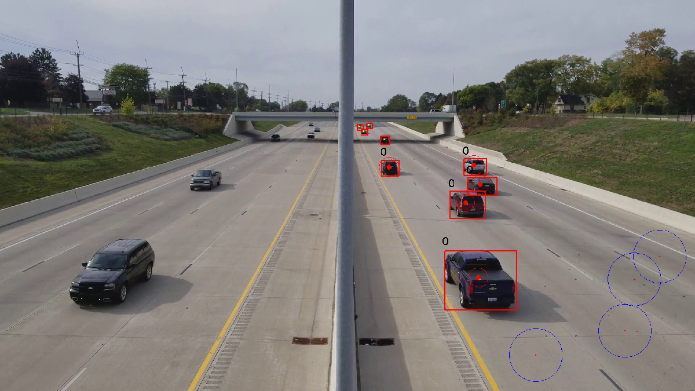
\includegraphics[width=0.85\linewidth]{../../../experiments/\Ex/\Vs/DINO/58}
        \caption{Frame number: 58.}
        \label{fig:\Ex-\Vs-\Set:06}
    \end{subfigure}
    \caption{Image sequence of tracked objects using GM-PHD filter with dynamic detection probability, Grounded SAM and adjusted models -- part 2.}
    \label{fig:\Ex-\Vs-\Set_2}
\end{figure}


Table \ref{tab:\Ex-\Vs-\Set_pd} displays values of detection probability of targets $C_L$ and $C_R$ in corresponding
frames. If the targets are visible in the scene, the detection probability is large. Once the targets are hidden
behind the obstacle, the detection probability rapidly drops. The value of the probability is about 0.1 from frame $
50$ to $54$. The effect of this low detection probability is projected in Table \ref{tab:\Ex-\Vs-\Set_w}. The targets'
weight is slowly decreasing, sustaining the targets' existence in period without any measurement.
\begin{table}[H]
    \centering
    \begin{tabular}{|c|c|c|}
        \hline
        Frame number & $C_L$ & $C_R$ \\ \noalign{\hrule height 1.5pt}
        44 & 0.934 & 0.861 \\
        \hline
        48 & 0.731 & 0.880\\
        \hline
        50 & 0.115 & 0.455\\
        \hline
        53 & 0.096 & 0.134\\
        \hline
        54 & 0.366 & 0.115 \\
        \hline
        58 & 0.924 & 0.940\\
        \hline
    \end{tabular}
    \caption{The evolution of detection probabilities of targets $C_L$ and $C_R$.}
    \label{tab:\Ex-\Vs-\Set_pd}
\end{table}

\begin{table}[H]
    \centering
    \begin{tabular}{|c|c|c|}
        \hline
        Frame number & $C_L$ & $C_R$ \\ \noalign{\hrule height 1.5pt}
        44 & 0.997 & 0.998 \\
        \hline
        48 & 0.998 & 0.999\\
        \hline
        50 & 0.872 & 0.970\\
        \hline
        53 & 0.628 & 0.618\\
        \hline
        54 & 0.998 & 0.541 \\
        \hline
        58 & 0.999 & 0.999\\
        \hline
    \end{tabular}
    \caption{The evolution of weights of targets $C_L$ and $C_R$.}
    \label{tab:\Ex-\Vs-\Set_w}
\end{table}

This experiment illustrates that even in scenarios with challenging conditions, such as angled recordings, it is
possible to configure the model using prior scene knowledge in a manner that enables the filter to effectively handle
obstacles obstructing the camera view.
Moreover, these model settings are capable of addressing the necessity for dynamically setting the noise covariances.
Tables \ref{tab:\Ex-\Vs-\Set_pd} and \ref{tab:\Ex-\Vs-\Set_w} demonstrate the effect of dynamic detection probability on targets' weights.
Note that targets
in Figures \ref{fig:\Ex-\Vs-\Set_1} and \ref{fig:\Ex-\Vs-\Set_2} are correctly in \textit{hidden} state, thus if the
obstacle would be larger, due to possibility of changing the pruning threshold for targets in \textit{detected} and \textit{hidden} state, the targets might survive for long period. This additional threshold possibility does not allow to create other false targets that would appear if the standard pruning threshold is lowered.